There are several types of low-level task the surgeon usually employs while
performing the surgery.
The most common:

\begin{description}
  \item Reconnection and joining of blood vessels to the arteries.

  \item[End to end aortoplasty:] the surgeon completely cuts away the
    affected part of aorta and sutures the two ends of aorta back together.

  \item[Patch aortoplasty:] the surgeon performs a cut along the axis of
    the aorta thus allowing the narrow place to expand. Then applies a
    patch from artificial material to fill the hole in.

  \item[Subclavian flap aortoplasty:] the nearest artery is cut,
    removing also half of the artery (along the axis) and part of the
    aorta in the affected place. He then uses the rest of the artery to
    patch the aorta.

\end{description}

With our method we are able to simulate all these tasks.
We have based our general approach on the common task involved in all these operations which is suturing of two or more edges together.
Since we are interested in predicting the result rather than creating a training simulator for suturing (trained surgeon knows well how to perform the sutures) the simplest way of performing the suture would be to connect the respective edges with springs. 
Springs however adds some unwanted energy to the system. 
Our method is based solely on the relaxation of the mesh of shell elements.
%% christian: I like the "relaxation" term !!!

We start with a mesh representing the situation after all the cuts have been performed but before suturing takes place. 
In the first step we perform the required topological changes to the mesh. We keep the number of elements in new mesh the same as in the original mesh so that we can define 1:1 mapping between elements of these meshes.
The Figure \ref{fig-JoiningVessels} explains this operation when joining vessels. 
Then we start the simulation on the modified mesh while using the original mesh to define rest shapes of all shell elements. 

\begin{figure}[tbh]
\begin{center}
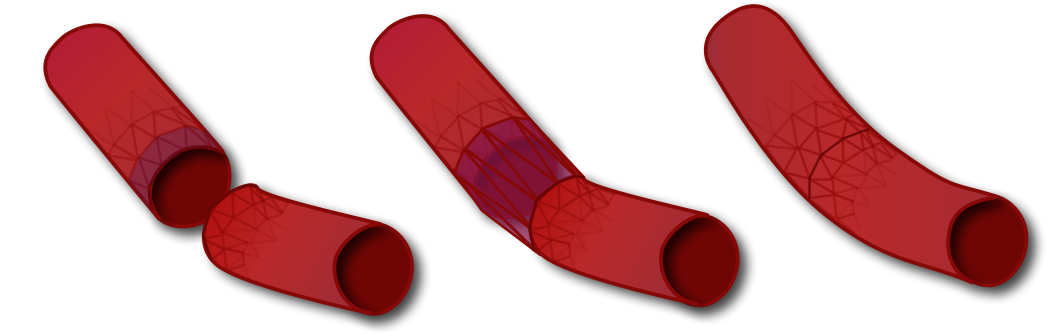
\includegraphics[width=\columnwidth]{img/rest_shape_scheme.png}
\end{center}

\caption{Scheme showing the method for joining two vessels. \christian{Do we need to extend the scheme for every type of aortoplasty (end to end / Patch / Subclavian): it would illustrate that the relaxation method works for every case...}
  \tomas{No we don't. This there will be real examples in results (if I remember correctly).} }
\label{fig-JoiningVessels}
\end{figure}

In case of non-trivial distance between the nodes that are sutured together the involved elements will undergo large deformation at the beginning of the simulation.
This results in quick increase of internal forces which can cause unwanted effects.
To allevieate the problem we have implemented the technique that allows for moderate changes in the rest shape between simulation steps.
Between the start and the end of the simulation we use a linear interpolation of the rest shape for the shells that lie along the sutured edges. 
\christian{I think that it is unclear that we do the relaxation on some shells that are on the side edges of the connecting line}
\tomas{I don't understand what do you mean by that. We will have to discuss that.}
The interpolation starts with the rest shape equal to the deformed elements and we progressively recontract the rest shape of the relaxed shells to their initial shapes. 
The energetical equilibrium found by the simulation gradually forces the side edges to connect.
After the mesh relaxes the simulation again terminates.

% vim: et sw=2 tw=0 spell
